% 熵
% 热力学|玻尔兹曼|熵|统计力学

\pentry{理想气体状态方程\upref{PVnRT}}
在热力学和统计力学中, \textbf{熵(entropy)}用于描述系统的无序程度, 是一个状态量, 通常记为 $S$. 例如若已知理想气体的 $P, V, n, T$ 等状态量, 就可以确定它的熵. %链接未完成

\subsection{宏观定义}

熵是一个系统的状态参量,它的增量为
\begin{equation}
\mathrm{d} S = \left . \frac{\Delta Q}{T}\right |_{\text{可逆}}
\end{equation}
其中,$\Delta Q$是可逆吸热,也就是说系统应无限地接近平衡态.

根据这个定义,经过任一卡诺循环,墒均回到初始值:
\begin{equation} \label{Entrop_eq1}
\sum{\text{d}S_i=0}
\end{equation}
然而,要成为真正意义上的「状态参量」的桂冠,\autoref{Entrop_eq1}应该对任何循环都成立,而不是只对卡诺循环成立.换言之,我们想要
\begin{equation}
\oint \mathrm d S =0
\end{equation}
对于所有循环均成立.这恰恰是正确的.这个证明基于这样的事实: 热不能全部变为功而不产生其他效果.因为它意味着$\eta=1$,违背了卡诺的结论.

\begin{figure}[ht]
\centering
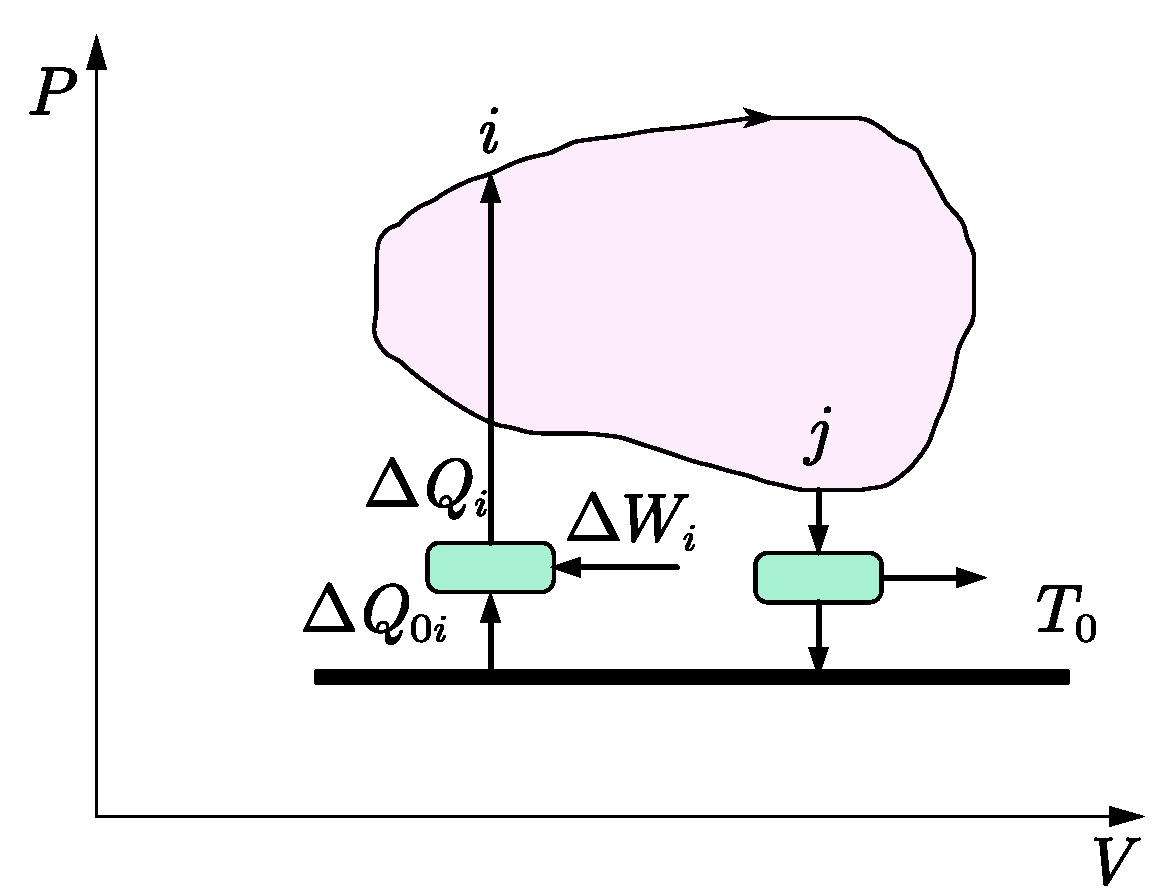
\includegraphics[width=8cm]{./figures/Entrop_1.pdf}
\caption{系统进行准静态循环} \label{Entrop_fig1}
\end{figure}

系统在$i$段吸热$\Delta Q_i$,该热量来自工作于系统现在的温度与热库$T_0$之间的卡诺制冷机.制冷机所需要的功是$\Delta W_i$.若$\Delta Q_i<0$,例如$j$点处,热量由卡诺热机出系统井向热库$T_0$放出该热量.

现在,我们证明,对于任意循环都有$\oint \mathrm d S =0 $.设系统经过如图所示的循环,图中有个温度为$T_0$的辅助热库.在循环上取一小段过程$i$.若此过程中的吸热为$\Delta Q_i$,则设想它是由一个卡诺制冷机供给的,这个制冷机工作于热库$T_0$和系统此时的温度$T_i$之间.工作过程中,制冷机从热库$T_0$吸收的热量为$\Delta Q_{0i}$,所需的功为$\Delta W_i$.卡诺制冷机满足
\begin{equation}
\frac{\Delta Q_{0i}}{T_0}=\frac{\Delta Q_i}{T_i}
\end{equation}
将之对闭合回路求和(在有些段,例如图中的$j$段,$\Delta Q_i$和$\Delta Q_{0i}$,可以是负值),得
\begin{equation}
\frac{Q_0}{T_0}=\oint{\frac{\text{d}Q}{T}}
\end{equation}
式中,$Q_0$是从那个热库吸收热量的总值.如果$Q_0$为零,我们就求得了所要的结果
\begin{equation}
\oint{\frac{\text{d}Q}{T}=\oint{\text{d}S=0}}
\end{equation}

我们将看到,的确如此(表示$\mathrm dS $时,我们用的是$\mathrm dQ/T$,而不是$\Delta Q/T$,因为该比值代表微分.)

如果$Q_0>0$,则意味着热库失去了热量.因为系统和所有辅助的卡诺机都已经复原,根据能量守恒,这部分热量一定由卡诺机和我们的系统全部转化为了等量的功,即$\eta=1$,而这是不可能的.如果$Q_0<0$,我们可以使整个过程反向进行(因为对于卡诺机和我们的循环,所有步骤都是可逆的),这样的$Q_0$符号就为正,出现如同前面一样的矛盾.

即使没有跟我们一起进行上面的证明,你也一定注意到了,如果要用$\Delta Q/T=\mathrm d S$将$\Delta Q$和$\mathrm dS$联系在一起,那么交换的热量$\Delta Q$必须是可逆的.

现在我们还没有完全了解$S$的意义,我们只知道它是个状态参量和它的定义式.下面我们来看一下它到底是啥:先改写一下热力学第一定律,采用$S$进行描述:
\begin{equation}
\mathrm d E = \dd{Q} - P\mathrm d V
\end{equation}
因为$E$是状态参量,因此$\mathrm d E$与热量如何进入系统无关.我们设热最的交换是可逆的,这样有
\begin{equation}
\mathrm d E =T\mathrm dS - P\mathrm d V
\end{equation}
从数学上讲,可以认为$E$是$S $和$V $的函数,且
\begin{equation}
T=\frac{\partial E}{\partial S}
\end{equation}
\begin{equation}
P=-\frac{\partial E}{\partial V}
\end{equation}
因为我们现在关注的是$S$,所以将第一定律写为
\begin{equation}
\text{d}S=\frac{1}{T}\text{d}E+\frac{P}{T}\text{d}V
\end{equation}
此方程告诉我们$S$(对于一定量的气体,如$197 \rm mol$)是宏观量的函数,如体积$V $、能量$U$,且
\begin{equation}
\left. \frac{\partial S}{\partial U} \right|_V=\frac{1}{T}\quad \left. \frac{\partial S}{\partial V} \right|_U=\frac{P}{T}
\end{equation}
要记住这两个方程.

在我们了解熵$S $的含义前,先利用下面这个公式,实际计算几个过程的熵变:
\begin{equation}
\left. \text{d}S=\frac{\text{d}Q}{T} \right|_{\text{可逆}}
\end{equation}

\begin{example}{质量为$m $的冰在$0^\circ\text{C}$时的熔化问题}
先看质量为$m $的冰在$0^\circ\text{C}$时的熔化问题.我们必须将潜热$L=80\rm cal/g$可逆地给系统,也就是用温度为$\left( 0+\varepsilon \right) ^\circ\text{C}\left( \varepsilon \rightarrow 0 \right)$热库为系统提供热量,使冰水混合物的系统充分吸热,达到水增多一点儿的新平衡态.一直这样做,直到所有的冰在此温度下全部熔化,
\begin{equation}
S_2-S_1=\int_1^2{\frac{\text{d}Q}{T}=\frac{mL}{T_\text{冰}}\left( \text{cal}/\text{K} \right)}
\end{equation}
式中,$T_\text{冰}= 237. 16\rm K $.

\end{example}
在这个简单的例子中,$ T $固定,等于$T_{\text{冰}}$,所以它可以提出到积分号的外面,积分的结果为$ml$.

接下来我们考虑稍微复杂一些的情况.

\begin{example}{将质量为$m $的水加热($T_1\to T_2$)}
将质量为$m$的水加热,使其温度由$T_1$升高到$T_2$.熵变为
\begin{equation}
S_2-S_1=\int_1^2{mc_{\text{水}}\frac{\text{d}T}{T}}=mc_{\text{水}}\ln \frac{T_2}{T_1}
\end{equation}
再次强调,记住热量应该可逆地进入系统:你不能将温度为$T_1$的水猛地倒入温度为$T_2$的锅中.相反,你将它与一连串的热库接触,每个热库的温度都比前一个热库的温度高一个无限小量,水有足够的时间与每个热库达到平衡,最终使水的温度从$T_1$升高到$T_2$.

如果你将水冷却降温,也可以用这个方程,但结果是负值,因为$T_2<T_1$.

最后我们计算气体的熵变,其结果非常有意义.温度为$T $的气体等温膨胀,体积从$V_1$增大到$V_2$,如图所示.
\begin{figure}[ht]
\centering
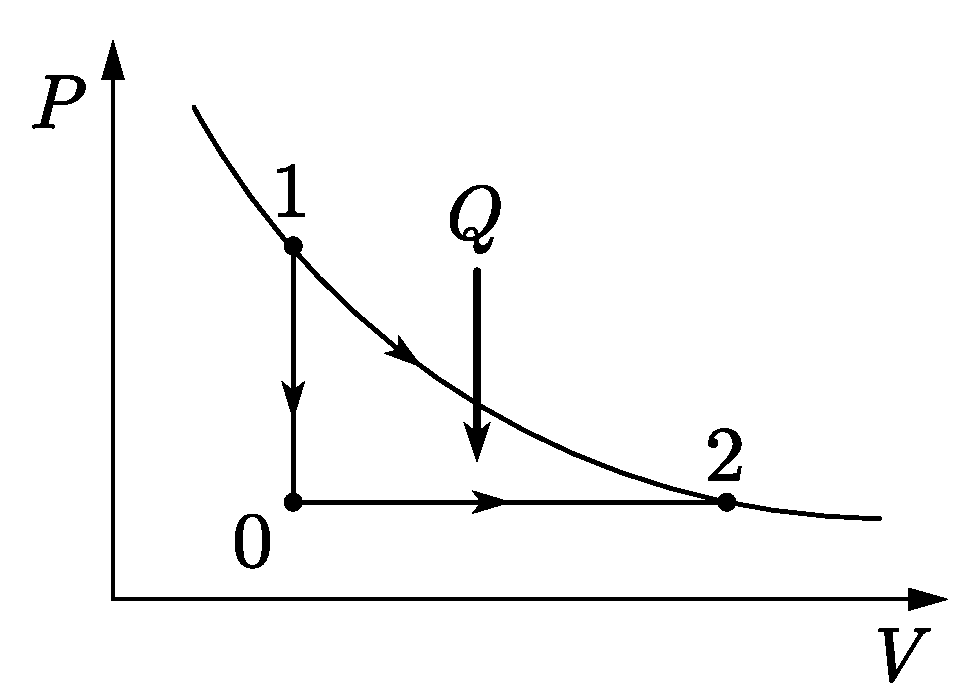
\includegraphics[width=5cm]{./figures/Entrop_2.pdf}
\caption{1、2点温度相同} \label{Entrop_fig2}
\end{figure}
\end{example}
与冰熔化时类似,温度$T $为常量,可以放到积分号的外面:
\begin{equation}
S_2-S_1=\int_1^2{\frac{\text{d}Q}{T}}=\frac{1}{T}\int_1^2{\text{d}Q=\frac{Q}{T}}
\end{equation}
式中,$ Q $是气体吸收的总热量.因为等温过程中$E$为定值,$Q$等于气体所做的功,因此
\begin{equation}
S_2-S_1=\int_1^2{\frac{\text{d}Q}{T}}=\int_1^2{\frac{P\text{d}V}{T}}=\int_1^2{\frac{nRT\text{d}V}{VT}=nR\ln \frac{V_2}{V_1}}
\end{equation}
如果每个点都有唯一的熵,那么$1$、$2$两点的熵差与我们怎样从$1$到达$2 $无关.因此,如果不沿等温路径的话,我们可以顺着$P $轴下降到达$0 $点,该点与$1 $点的体积相同,即$V_0=V_1$且$P_0=P_2$.熵变为
\begin{equation}
S_{0}-S_{1}=n c_{v} \int_{T_{1}}^{T_{0}} \frac{\mathrm{d} T}{T}=n \frac{3 R}{2 |} \ln \frac{T_{0}}{T_{1}}=n \frac{3 R}{2} \ln \frac{T_{0}}{T}
\end{equation}
\begin{equation}
S_{2}-S_{0}=n c_{p} \ln \frac{T_{2}}{T_{0}}=n \frac{5 R}{2} \ln \frac{T}{T_{0}}
\end{equation}
\begin{equation}
\begin{aligned} S_{2}-S_{1} &=n \frac{3 R}{2} \ln \frac{T_{0}}{T}+n \frac{5 R}{2} \ln \frac{T}{T_{0}} \\ &=n \frac{3 R}{2} \ln \frac{T_{0}}{T_{0}}+n \frac{2 R}{2} \ln \frac{T}{T_{0}}=n R \ln \frac{T}{T_{0}} \\ &=n R \ln \frac{V_{2}}{V_{1}} \quad\left(\text { 用到了 } \frac{T}{T_{0}}=\frac{T_{1}}{T_{0}}=\frac{P_{1} V_{1}}{P_{0} V_{0}}=\frac{P_{1}}{P_{2}}=\frac{V_{2}}{V_{1}}\right) \end{aligned}
\end{equation}
这里用到了由\autoref{Entrop_fig2}得到的许多等式:$T=T_{1}=T_{2}, \quad V_{1}=V_{0} \text { 和 } P_{0}=P_{2}$.因此,求熵变时,我们可以随意选择路径.通常,我们选择最容易的路径.


\subsection{微观定义} 
\begin{equation}
S = k_B \ln \Omega
\end{equation}

% 举例: 高温物体热传导给低温物体, 损失多少?
 
% 未完成: 热机中熵如何变化? 等压等温绝热过程中熵如何变化?
